\subsection{change priors and chain initialisation}
A similar experiment is carried out as in \hyperref[nr obs]{\textcolor{blue}{Section }\ref{nr obs}}. Instead of changing the number of observations, the priors and chain initialisation are changed, investigating the effect on the posterior. Additionally, scaling of the parameters is applied, this is considered good practice and can improve numerical stability. 

\subsubsection{check seeds}
\textit{confirm all seeds are useful / coded correctly. I think I might have one too many.}


\subsubsection{the priors}
In previous sections of the logbook the prior for all parameters is N(10,10). This is slightly more informative than the uniform priors that are used conventionally in hydrology/hydrogeology, e.g. \cite{vrugt2009accelerating}.  Usually, a better estimate can be given, based on material brought to the surface during the creation of the piezometer borehole. The 'true' hydraulic conductivities of the models I designed range from 0.01 m/d up to 10 m/d. These values are typical for sediments found in lowland areas (\hyperref[fig_logbook8_k]{\textcolor{blue}{Figure }\ref{fig_logbook8_k}}). 

\begin{figure}[ht]
\centering
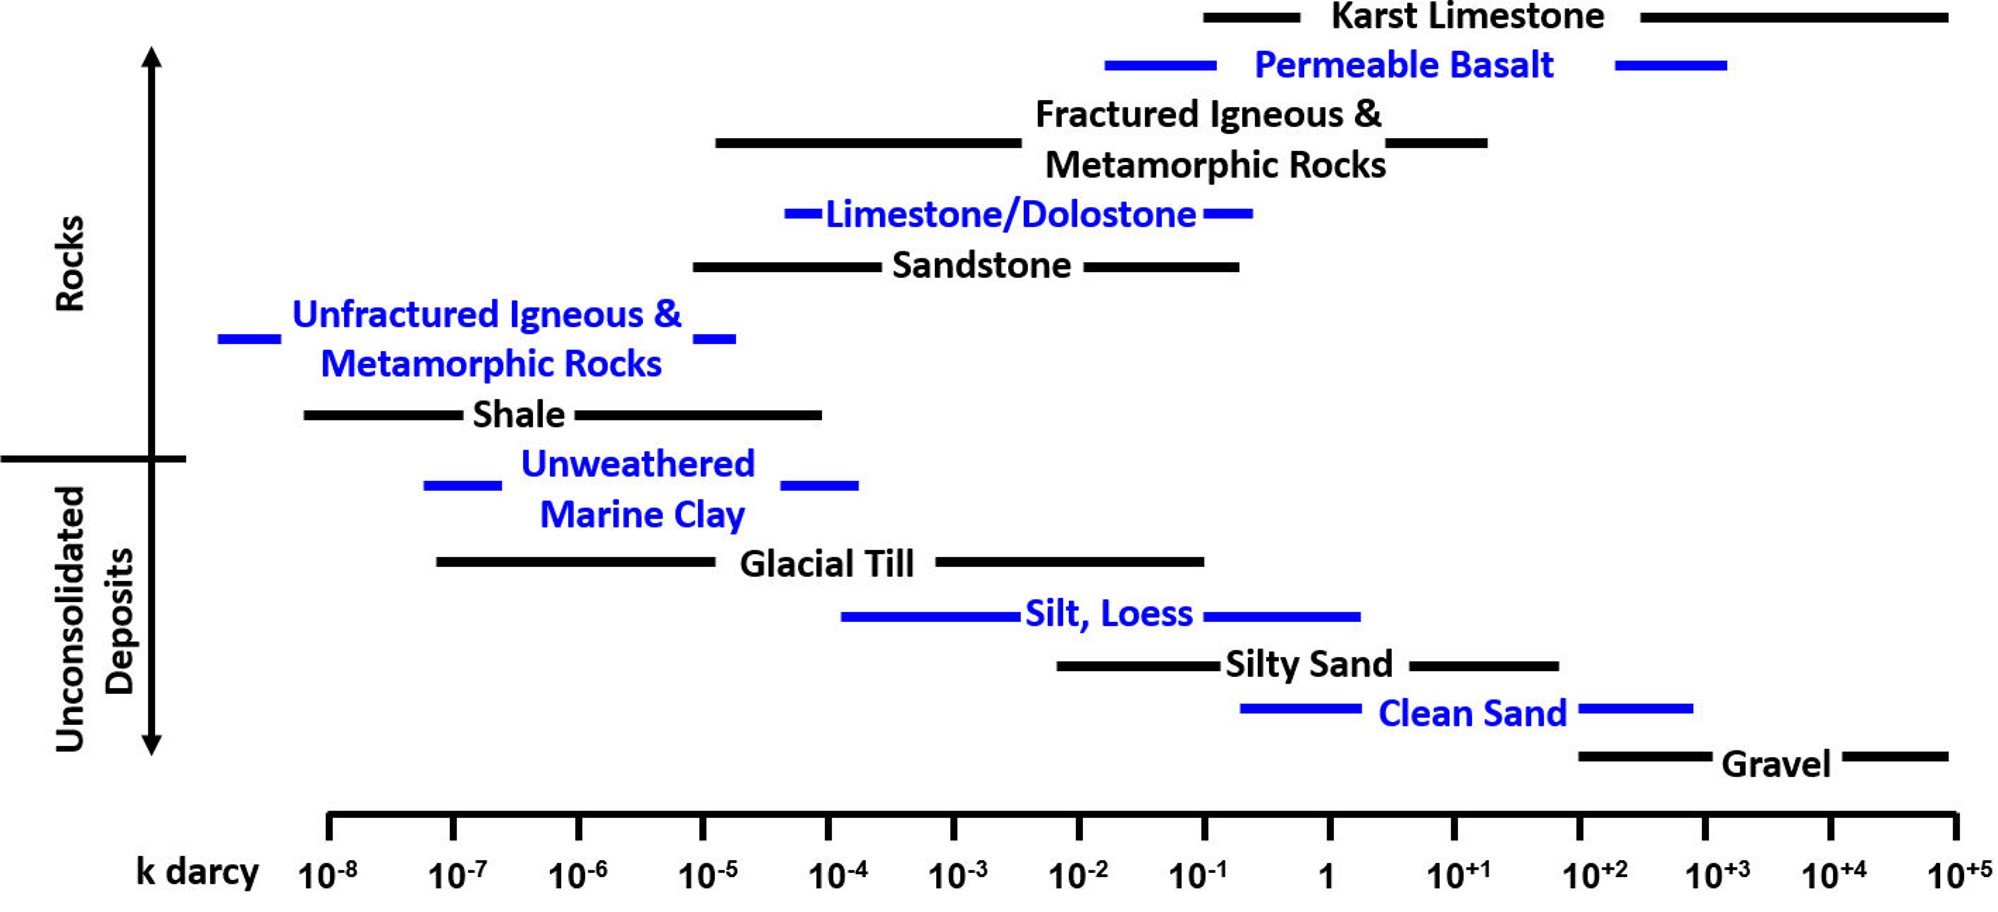
\includegraphics[width=1.0\textwidth]{Figures/appendix_figs/logbook8_hydraulic_conductivity_range.jpg}
\caption{Ranges of hydraulic conductivity values (m/d) of unconsolidated material, sedimentary rocks, and igneous and metamorphic rocks. The alternating colours are used to make the chart easier to read. This figure is adapted from \cite{woessner2020hydrogeologic}}\label{fig_logbook8_k} %so the location of the label influences how it is referenced!?, that's clunky
\end{figure}

To investigate the importance of prior selection, the obtained posterior when using Uniform priors is compared to the obtained posterior using Gaussian priors. Where, Gaussian priors are considered more informative, because typically extremes values are rarer. %Though I am not sure how it is distributed considering grain sizes and heterogeneity in case of Glacial material. So I'm assuming extremes are less common, but not super sure
For my synthetic models it is assumed that the lithology is known from drilling boreholes for the piezometers. Different Gaussian priors were designed for different lithologies, based on typical sediments found in lowland areas and their hydraulic conductivity (\hyperref[fig_logbook8_k]{\textcolor{blue}{Figure }\ref{fig_logbook8_k}}), resulting in the priors presented in \hyperref[tab_logbook8_priors]{\textcolor{blue}{Table }\ref{tab_logbook8_priors}}. 
Parameters were limited to values inside the range given by the Uniform priors of the respective lithology. With the package emcee such parameter limits are implemented by having the function which computes the logposterior return negative infinity (\href{https://emcee.readthedocs.io/en/stable/user/faq/}{emcee})

\begin{table}[ht]
\centering
\caption{Priors for the hydraulic conductivities of three different sediments found in Model 1 to 4. For each sediment a uniform prior and a Gaussian prior has been designed. For the Gaussian priors 99.7\% ($3\sigma$) of all probability mass is within the same range as defined by the Uniform priors}
\label{tab_logbook8_priors}
\begin{tabularx}{\textwidth}{XXX}
\toprule
Sediment & Uniform Prior (m/d) & Gaussian Prior log(m/d)\\
\midrule
Clean Sand & Unif($10^{-1}, 10^3$) & N( 1, 0.67)  \\
Silty Sand  & Unif($10^{-2}, 10^2$) & N( 0, 0.67) \\
Silt, Loess   & Unif($10^{-3}, 10^1$)  &  N(-1, 0.67) \\
\bottomrule
\end{tabularx}
\centering
\end{table}

\subsubsection{initialisation}
Observation: very large steps take place (reference a trace plot), as a consequence outlier chains come into existence. When all other chains have converged, no big steps toward the typical set is possible, due to how the DE moves work (maybe this is actually possible for the stretch move, that would be a pretty big advantage). 

Hypothesis: This can be solved by making the initialisation less dispersed, resulting in smaller initial steps (a possible drawback would be that it may take longer to reach the typical set, if initialisation is far from typical set).

\subsubsection{scaling}
In chapter C8, chains struggled to reach the value of 0.01 of $\theta_4$. This may be caused by it being so close to 0 and all proposals below 0 to be rejected. Additionally, moves are effectively a fancy interpolation, so overshooting 0 when parameters are still nonzero is very likely and the new proposal may be in the opposite direction, causing the chain to move away from 0 again towards even larger non-negative values. 